%\documentclass[a4paper,ngerman,titlepage]{scrartcl}
\documentclass[a4paper,english,titlepage]{scrartcl}

\def\myauthor{}
\def\mytitle{XeTeX template}
\def\mycopyright{\myauthor}
\def\mykeywords{}
\def\mysubtitle{}
\def\myemail{}
\def\myweb{}
\def\myphone{}

\usepackage{unicode-math}
\usepackage{amsmath}
\usepackage{xunicode}
\usepackage{xltxtra}

%use default serif font for headlines, title etc. instead of koma script's default font
\addtokomafont{disposition}{\rmfamily}
\setromanfont{TeX Gyre Pagella}
%\setromanfont[Mapping={tex-text},Numbers={OldStyle},Ligatures={Common}]{Minion Pro} 
\setsansfont[Mapping=tex-text,Colour=AA0000]{Myriad Pro}
\setmonofont[Mapping=tex-text,Scale=1.0]{Inconsolata} 
\setmathfont{Asana Math}

\usepackage{listings}
\usepackage{fancyhdr}
\usepackage{babel}
\usepackage{textcomp}
\usepackage{graphicx}
\usepackage{natbib} %todo
\usepackage{color}

\pagestyle{fancy}

\usepackage[xetex, 
	colorlinks=false,
	urlcolor=BlueViolet,
	plainpages=false,
  pdfpagelabels,
  bookmarksnumbered,
  pdftitle={\mytitle},
  pagebackref,
  pdfauthor={\myauthor},
  pdfkeywords={\mykeywords}
]{hyperref}

\definecolor{dkgreen}{rgb}{0,0.6,0}
\definecolor{gray}{rgb}{0.5,0.5,0.5}
\definecolor{mauve}{rgb}{0.58,0,0.82}
%\definecolor{listingbg}{rgb}{0.93,0.95,0.9}
\definecolor{listingbg}{rgb}{0.99,0.99,0.99}

\lstset{
	tabsize=2,
	rulecolor=,
 	basicstyle=\scriptsize,
	numbers=left,
	numberstyle=\tiny\color{gray},
  stepnumber=1,
  numbersep=5pt,
  backgroundcolor=\color{listingbg},
	upquote=true,
  frame=single,
  rulecolor=\color{black},
  captionpos=b,
	columns=fixed,
	showstringspaces=false,
	extendedchars=false,
	breaklines=true,
	prebreak = \raisebox{0ex}[0ex][0ex]{\ensuremath{\hookleftarrow}},
	showtabs=false,
	showspaces=false,
	showstringspaces=false,
	identifierstyle=\ttfamily,
  keywordstyle=\color{blue},
  commentstyle=\color{dkgreen},
  stringstyle=\color{mauve},
}

\begin{document}

\title{\mytitle}
\author{\myauthor}

\maketitle
\tableofcontents{}

\newpage{}

\section{Section 1}
\label{sec:Section1}

\subsection{Subsection 1}
\label{sec:Section1_1}

\cite{Stronger2006}

\begin{enumerate}
\item Item1
\item Item2
\item Item3
\end{enumerate}

\begin{itemize}
\item Item1
\item Item2
\item Item3
\end{itemize}

\begin{lstlisting}[language=Python, caption=Python source, label=PythonCode]
for i=1 to numIterations do:
	# doSomething
  doSomething()

return X
\end{lstlisting}

\lstinputlisting[language=Java, caption=Java source from external file, label=JavaCode]{src/test.java}

\ref{sec:Section1}

\begin{center}
$m(line)=\frac{f_{\theta}\left(1-\frac{\theta}{180}\right)+f_{l}\left(1-\frac{l}{\sqrt{x_{img}^{2}+y_{img}^{2}}}\right)+f_{o}\left(\frac{o}{l_{ex}}\right)+f_{d}\left(1-\frac{d_{1}+d_{2}}{2\sqrt{x_{img}^{2}+y_{img}^{2}}}\right)}{f_{\theta}+f_{l}+f_{o}+f_{d}}$
\par\end{center}

\begin{center}
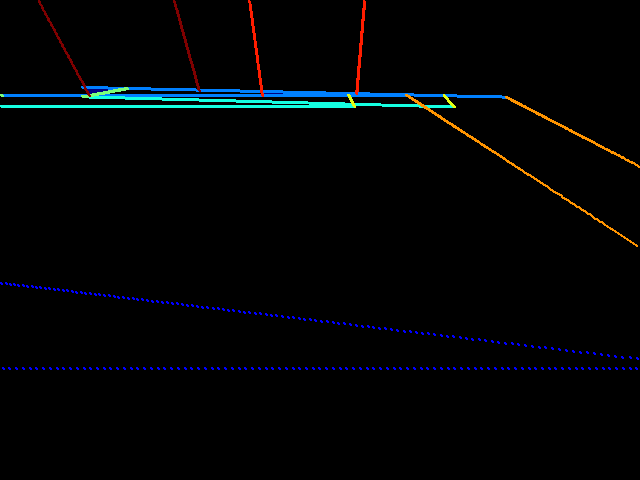
\includegraphics[width=0.3\textwidth]{img/test}
\par\end{center}

\clearpage{}

\section{Section 2}
\label{sec:Section2}

\clearpage{}

\bibliographystyle{plain}
\bibliography{xetex-template}

\end{document}
